\subsection{\textbf{Eventos Importantes:}}

\subsubsection{\textbf{O que é o Evento \textit{Halving}?}}
O evento Halving é um acontecimento periódico em que o número de Bitcoins em cada bloco minerado é reduzido pela metade, ocorre especificamente a cada 210 mil blocos minerados. Apesar de sua data não ser totalmente certa, é possível estimar com grande precisão, normalmente ocorrendo a cada 4 anos.

Seu objetivo é tentar controlar o valor da moeda com a inflação. O Halving não tem relação direta com a intenção de aumentar diretamente o valor de mercado da moeda, suas intenções valem tentativa de controle sobre o valor da moeda com a inflação. Adicionando o fato de que seu(s) criador(es) já deixaram bem explícito que haverá uma quantidade limitada de unidades de Bitcoin, o que já está fixo na quantidade de 21 milhões.

Os efeitos do halving influenciam em seu valor indiretamente, já que pela lei da oferta e demanda, com a queda da oferta sobre o Bitcoin e que normalmente há um aumento na demanda, seu preço aumenta.

Ele já ocorreu 4 vezes. Em 28 de novembro de \textbf{2012}, 9 de julho de \textbf{2016}, 11 de maio de \textbf{2020}  e 19 de abril de \textbf{2024}

% Tabela da Linha do Bitcoin Halving 
\begin{figure}[h]
    \centering
    \shadowbox{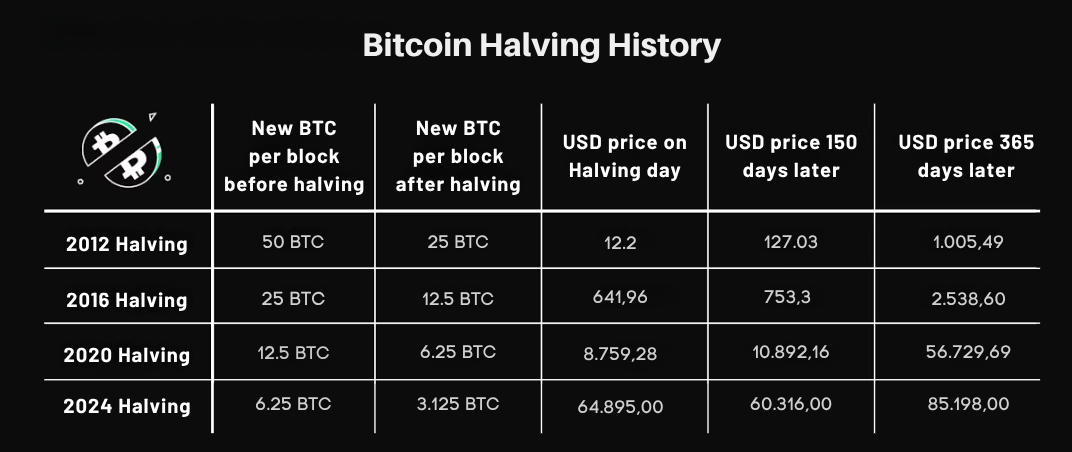
\includegraphics[width=0.8\textwidth]{Imagens/Tabela_Halving.png}}
    \caption{Tabela Cronológica do Evento Halving}
    \label{fig:Tabela Cronologica do Evento Halving}
\end{figure}

\subsubsection{\textbf{A Queda da Mt. Gox}}
Em 2006, a empresa \textit{Magic: The Gathering Online Exchange}, ou mais conhecida por somente \textbf{Mt. Gox}, fora criada por Jed McCaleb com o objetivo de ter uma plataforma de troca de cartas de um jogo online chamado \textit{Magic: The Gathering Online}.  Contudo, em 2010, começou a entrar no ramo de mineração de Bitcoin, rapidamente tornando-se a maior corretora no mercado de criptomoedas, conseguindo ter a maior Exchange (plataformas de transações de criptomoedas) de Bitcoin no Mundo inteiro.  Em seu auge — no ano de 2013 — ela administrava mais de 70\% das transações em Bitcoin no mundo. 

No entanto, essa dominância no mercado não permaneceu por muito temo. Em \textbf{07 fevereiro de 2014}, a corretora alegou problemas técnicos e suspendeu os saques de Bitcoin. Em \textbf{24 de fevereiro} ocorreu Fechamento de sua \textit{Exchange} e logo em seguida, em \textbf{28 de Fevereiro}, a Mt. Gox declarou falência. Expondo uma perda de cerca de 850 mil Bitcoins — Aproximadamente 450 milhões de dólares na época. Essa perda provocou uma queda no valor do Bitcoin em quase 36\% entre fevereiro e março do mesmo ano. 

% Gráfico sobre o Impacto da Mt. Gox
\begin{figure}
    \centering
    \shadowbox{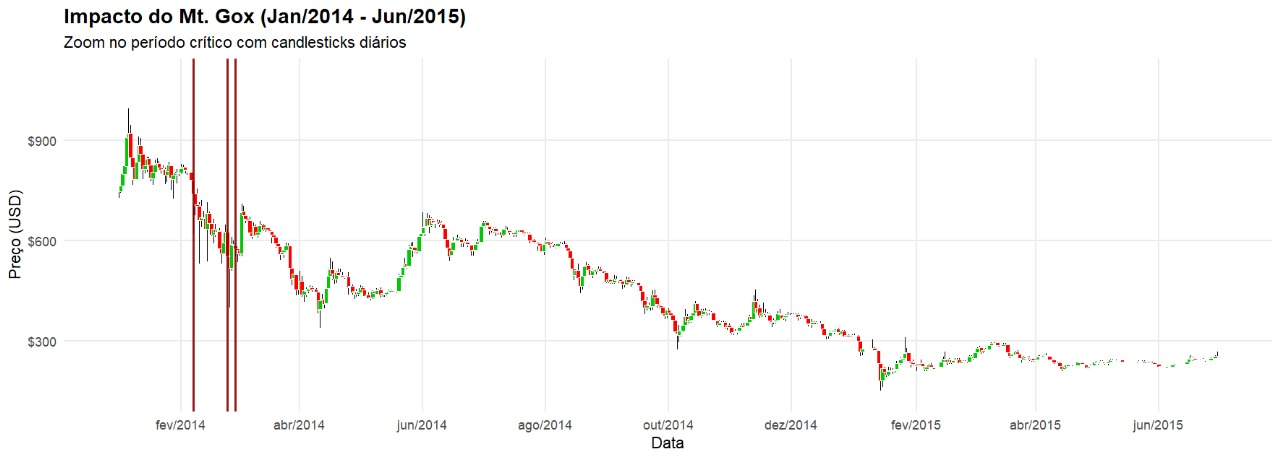
\includegraphics[width=1\textwidth]{Imagens/Mt_Gox_Grafico.jpg}}
    \caption{Impacto da Mt. Gox}
    \label{fig:Mt. Gox Gráfico}
\end{figure}

Posteriormente, a empresa encontrou 200 mil Bitcoins (dos 850 mil perdidos) em carteiras frias — dispositivos offline para armazenamento seguro, porém a perda total ainda permanece como um dos maiores desastres financeiros no ramo das criptomoedas. O motivo dessa perda pela empresa forem vindos de uma má gestão da plataforma, agravada por falhas no sistema de segurança. Acredita-se que hackers russos foram retirando Bitcoins de forma gradual, explorando as brechas na segurança. 
 \newpage
A quebra da Mt. Gox abalou  significativamente a comunidade Bitcoin. Comprometendo a credibilidade nas corretoras de criptomoedas, impactando esse mercado que ficou cravado no público por anos. Esse episódio foi um alerta indesejado sobre a vulnerabilidade que tinha nesse mercado,  evidenciando a necessidade de fortalecimento de práticas de regulação para proteger os investidores para reatar a confiança no mercado cripto.

\subsubsection{\textbf{Pandemia COVID-19}}

No começo da pandemia de COVID-19, houve um caos generalizado junto com uma transformação abrupta do cotidiano. Nenhum setor ficou isento de alterações, incluindo o ramo financeiro de criptomoedas. Assim como as moedas estatais e tradicionais, o Bitcoin também foi afetado e teve uma desvalorização de até 50\% de seu valor. Entretanto, com os governos aumentando a emissão das moedas fiduciárias, o Bitcoin se fortaleceu como um ativo de proteção contra inflação, conseguindo recuperar e alcançar seu preço máximo em 2021, ou pelo até o ano de 2024, que teve mais uma grande serie de aumento de seu valor.

% Gráfico Pandemia

\begin{figure}[h]
    \centering
    \shadowbox{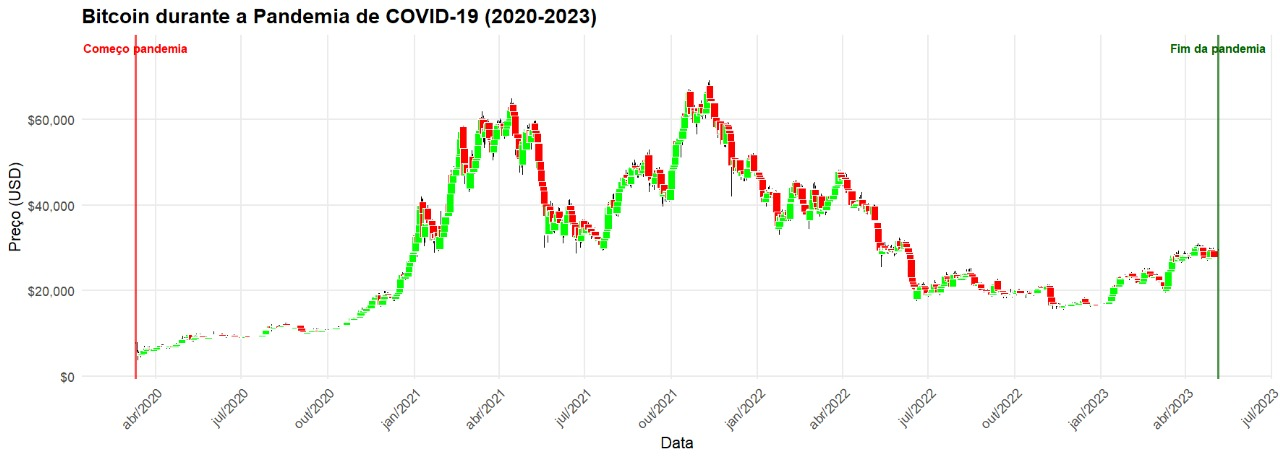
\includegraphics[width=0.8\textwidth]{Imagens/grafico_pandemia.jpg}}
    \caption{Bitcoin na Pandemia}
    \label{fig:pandemia}
\end{figure}

Vemos na \cref{fig:Candle Graph}, que logo no começo de 2020 temos um crescimento no valor de moeda do Bitcoin, devido ao pré-Halving. Assim como foi previsto, em 11 de maio aconteceu o evento halving. Porém, vemos também uma queda logo em seguida, representando a queda na economia global. Porém, pouco tempo depois já houve uma crescente em seu valor, representando na indução de um ativo contra a inflação.

\newpage 

Essa serie de aumento e redução de preços são variadas. Como falado, a desvalorização se deve a crise financeira mundial em conjunto com a pandemia COVID-19. Porém, sua valorização é mais devido à percepção de uma forma de proteção e diversificação para empresas e pessoas ainda conseguirem um meio viável de continuar com transações cotidianas. Por conta disso, a utilização de criptomoedas foi ampliado, entrando no cotidiano a fundo dessa vez. A integração de criptomoedas na forma de pagamento impactou o mundo, além de impulsionar o valor do Bitcoin.

Apesar de sua alta com o grande aumento do seu valor, o bitcoin acabou consolidando-se como “ouro digital”, ganhando destaque como um dos principais investimentos alternativos no mercado financeiro.

\subsection{\textbf{Material utilizado:}}

O banco de dados, “Bitcoin Historical Data”, que fora extraído da plataforma Kaggle, armazena todos os dados da história do Bitcoin em intervalos de 1 minuto, extraídos de Exchange de Bitcoin — plataformas de transações específicas para criptomoedas — onde as negociações ocorrem.	

O arquivo está no formato \texttt{.csv}, apresentando 6 colunas com variáveis numéricas em formato decimal, sendo separadas por ponto. O tamanho do arquivo é de 369.29 MB. Cobrindo o período de 1 de janeiro de 2012 até o presente, recebendo atualizações diárias para inclusão de novos dados. Entretanto, para a análise dos dados, o banco de dados será restringido até a  data de 01 de Junho de 2025.

\subsubsection{\textbf{As principais variáveis:}}

\begin{itemize}
    \item \textbf{Timestamp}: Indica a hora de início do tempo de 60 segundos, no horário Unix — tempo em segundos desde 1 de janeiro de 1970.
    \item \textbf{Open, High, Low e Close}: mostram como o preço se comportou no período de um minuto:
    \begin{itemize}
        \item \textbf{Open}: Preço de abertura na janela de tempo inicial.
        \item \textbf{High}: Preço mais alto na janela de 1 minuto.
        \item \textbf{Low}: Preço mais baixo na janela de 1 minuto.
        \item \textbf{Close}: Preço no fechamento da janela de tempo inicial.
    \end{itemize}
    \item \textbf{Volume}: Volume de BTC negociados nesta janela de tempo.
\end{itemize}

\subsection{\textbf{Metodologia:}}

A análise foi realizada na linguagem \texttt{R}, versão \texttt{4.5.0}, utilizando diversos pacotes para a manipulação e visualização dos dados. No dataset, os dados são distribuídos em intervalos de 1 minuto, porém para facilitar a análise, os dados foram agrupados por dia — mas sem alterar o seu conteúdo, para melhor visualização nos gráficos.

Para a limpeza e manipulação das amostras, foram utilizados os pacotes \texttt{tidyverse}, \texttt{magrittr}, \texttt{tidyquant} e \texttt{lubridate}. O \texttt{tidyverse} inclui o \texttt{dplyr}, utilizado para filtragem e agrupamento dos dados; o \texttt{lubridate} foi empregado para a conversão do timestamp; enquanto \texttt{magrittr} e \texttt{tidyquant} foram usados para facilitar a manipulação e as análises financeiras dos dados.

Para a criação dos gráficos foi utilizado o \texttt{ggplot2}, \texttt{tidyquant} e \texttt{scales}, para a elaboração de \textit{candlesticks} e linhas, que auxiliam a interpretação do comportamento do preço do Bitcoin. Além disso, para alguns cálculos financeiros e análise de desempenho, foram utilizados os pacotes \texttt{quantmod}, \texttt{TTR} e \texttt{PerformanceAnalytics}.

Fora criado gráficos de candlestick  para melhor visualização do historico de valor do Bitcoin ao decorrer dos anos. Focando tanto em eventos específicos, como a queda da Mt. Gox, quanto ampliando para o período completo para melhor noção geral. Além de utilizar gráficos de dispersão para analises de correlação e melhor discernimento do comportamento humano em relação ao Bitcoin.